\documentclass[article]{proc}
\usepackage{abstract}
\renewcommand{\abstractname}{}    % clear the title
\renewcommand{\absnamepos}{empty} % originally center

\titleConf{DAII\\
December 13th, 2019}
\city{Austin, TX, USA}
\usepackage{color}
\usepackage{graphicx}
\begin{document}
%%%%%%%%%%%%%%%%%%%%%%%%%%%%%%%%%%%%%%%%%%%%%%%%%%%%%%%%%%%%%%%%%%%%%%%%%%%%%%%%%%%%%%%%%%%%%%%%
\title{A quantitative framework for fire department unit purchasing decisions}
%For at least  authors with different addresses, use instead the following commands
\corrauthor[1]{Tyler C. Buffington}
\corremail{tyler.c.buffington@utexas.edu}
% \doi{http://dx.doi.org/10.1615/TFESC.XXX.XXX}
\address[1]{The University of Texas at Austin, Austin, TX, 78712, USA}

\maketitle
%%%%%%%%%%%%%%%%%%%%%%%%%%%%%%%%%%%%%%%%%%%%%%%%%%%%%%%%%%%%%%%%%%%%%%%%%%%%%%%%%%%%%%%%%%%%%%%%



\section{Introduction}
The decision to purchase these units involves spending hundreds of thousands of dollars, and the outcomes are prone to large amounts of uncertainty due to the variability of fire/EMS incident trends. The purpose of this report is to describe a quantitative analysis of a unit purchasing decision that a fire department might face. The analysis involves using actual operational data for a real fire department, but the identity of the department is not disclosed due to confidentiality concerns. The example decision involves determining how to allocate up to \$1,000,000 to purchasing additional units. Although many departments have specialized units, this analysis is limited to Advanced Life Support (ALS) units and fire suppresssion units. The purpose of the ALS units considered in this project is to transport a patient in need of medical attention to a hospital as soon as possible. These units usually are staffed by 2-3 firefighters, and require that at least one of them is also a certified paramedic. These units also have additional medical equipment on board and can give medical treatment to patients before they arrive to the hospital. These units usually cost around \$300,000-\$500,000 each. Fire suppression units include several different units intended for different purposes. The most basic suppression unit is a fire engine, which contains a supply of water for fighting fires and they usually cost around \$800,000-\$1,000,000 each. Another common fire suppression unit is a ladder truck, which contains a ladder for firefighting and ventilation control in elevated spaces and they often cost over \$1,000,000 each. Generally, a fire station will include one ALS unit and one fire suppression unit, assuming that the fire department also handles EMS incidents in addition to fire incidents. The department used for this analysis has exactly one fire suppression unit and one ALS unit for each station at the time the data was used. 

Originally, the purchase of a ladder truck was considered as an alternative in the decision. However, after having three conversations with a Business Process Analyst of a fire department, we revised the strategies under consideration. He said that the capabilities unique to a ladder are used relatively infrequently (i.e. high rise fires), and so it is unlikely that a fire department would need an additional ladder truck if it already has more than one. The department used in this analysis has three ladder trucks, so purchasing an additional one was excluded from consideration. Due to the fact that roughly 80\% of the incidents a department responds to are medical, fire suppression units are most often used merely to transport firefighters to the scene of the incident so they can administer basic medical care as soon as possible. If the situation is serious enough, then an ALS unit will often come later to transport the patient to the hospital. As a result, all fire suppression units are lumped together for the purposes of this analysis.

In our conversations, the Business Process Analyst also stated that he believes that most fire departments are in need of more ALS units rather than more fire suppression units. He said that this is because response time is generally more important for ALS units given that their unique features are required for far more calls than fire suppression units. The nature of their calls is often more time-sensitive. In light of these conversations, the most viable alternatives are likely to be those involving purchasing ALS units, but the question of which stations should house them is not as straightforward. For the assumed \$1,000,000 budget, we assume that we can either purchase a new fire suppression unit or up to two new ALS units.

\section{Modeling methodology}
\subsection{Data processing}
The starting point for the modeling effort described in this report is a large dataframe of incident data containing information on over 82,000 unit dispatches that occurred between May of 2015 and November of 2019. Each row of this dataframe is a dispatch of either an ALS or a suppression unit. The columns of the dataframe correspond to the unit id, the unit type, the time the unit was dispatched, the time the unit was cleared from the incident, where the incident occurred, and the station that houses the unit. Based on the location of the incident, each row also contains a \textit{first due} station entry. This entry is based on the fact that the department's jurisdictional region is divided into six smaller non-overlapping regions (one for each station) that each comprise the set of locations that are assigned to a station. Loosely speaking, the first due assignments are based on distance, meaning that for example, Station A's first due area is the set of locations that are closer to Station A than any other station. However, other factors affect these assignments and the boundaries of the first due areas are considered a ``take as given" for the purposes of this project.


The first step was to split the dataframe into two separate dataframes- one containing only ALS units and one containing only fire suppression units. Then each dataframe was grouped by the first due station corresponding to the location of the incident. For each station and each unit type, two response time arrays were generated- one corresponding to units that belong to the first due station, and one corresponding to units that came from other stations. These distribution comparisons are shown in Figure \ref{fig:alsdiff} for ALS units and fire suppression units in Figure \ref{fig:firediff}.


\begin{figure}[!htb]
  \centering
  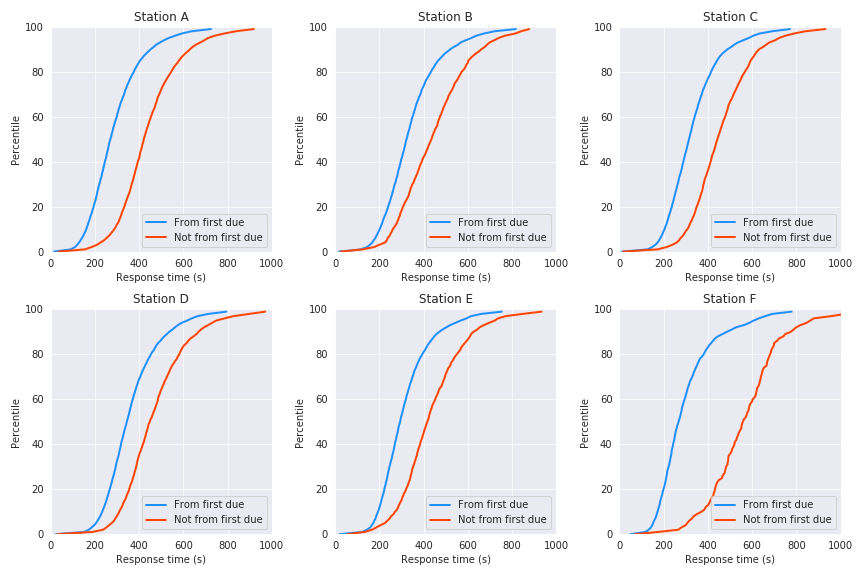
\includegraphics[width=16cm,keepaspectratio]{Figures/alsdiff.png}
  \caption{A comparison of the ALS response time distributions between cases when the unit is from the first due area vs. when the unit is not from the first due area, broken down by each first due area.}
  \label{fig:alsdiff}
\end{figure}

\begin{figure}[!htb]
  \centering
  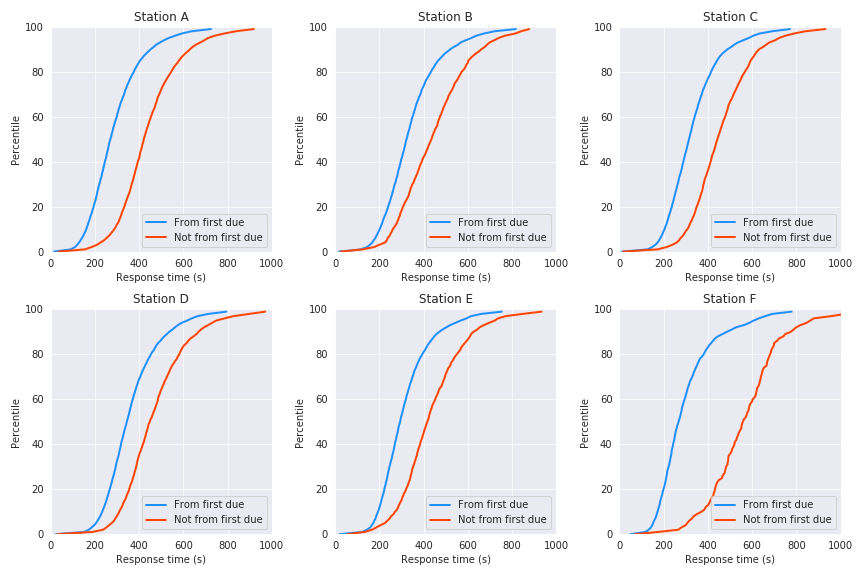
\includegraphics[width=16cm,keepaspectratio]{Figures/alsdiff.png}
  \caption{A comparison of the suppression response time distributions between cases when the unit is from the first due area vs. when the unit is not from the first due area, broken down by each first due area.}
  \label{fig:firediff}
\end{figure}

Then, the probability of a unit being sent to an incident occurring in each first due area was calculated along with the probability that the unit was sent from the first due station. Based on these probabilities, one can imagine a simplified probability tree like the one shown in Figure \ref{fig:alstree}. 

\begin{figure}[!htb]
  \centering
  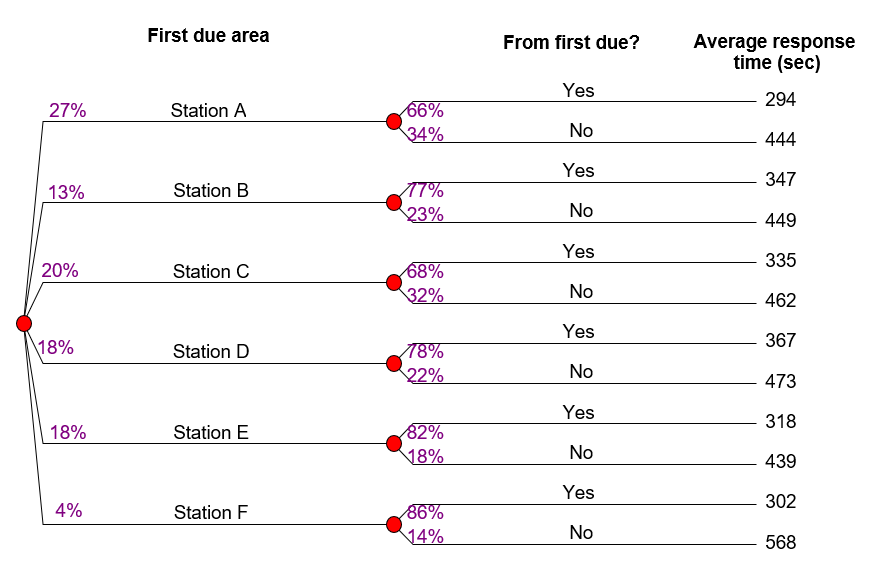
\includegraphics[width=16cm,keepaspectratio]{Figures/alstree.PNG}
  \caption{A simplified probability tree showing the main uncertainties relevant to the project. The values shown are the actual values for ALS units. Note that the average response times are shown for simplicity. In reality each of these is a distribution.}
  \label{fig:alstree}
\end{figure}

Based on the tree shown in Figure \ref{fig:alsdiff}, the effect of additional units can be modeled as a change to the ``From first due?" probability. In general, units are dispatched from non-first-due stations because the first due station does not have enough units to respond adequately. As a result, the effect of new units can be simulated by exploring the frequency of units being required in first due areas of stations while the first due station is out of units of the specified type. In order to do this, the author built an algorithm that iterates through each dataframe and determines the units of the same type that were active at the moment each unit was dispatched; active means that a unit is between its dispatched timestamp and its cleared timestamp.
As a simple example, one can imagine three hypothetical unit dispatches- Unit A, which is dispatched at 12:00 PM and cleared at 1:00 PM, Unit B, which is dispatched at 12:30 PM and cleared at 1:30 PM, and Unit C, which is dispatched at 12:45 PM and cleared at 2:00 PM. Assuming these three dispatched comprise the entire dataset, then for Unit A, the algorithm would determine that no units were active at the time Unit A was dispatched. For Unit B, it would identify that Unit A was active at the time of dispatch, and for Unit C, it would identify that both Unit A and Unit B were active at the time of dispatch. 

It is important to note that a unit can be unavailable even though it is not responding to an incident. For example, a unit can be taken out of service for maintenance. In order to estimate the frequency that units are unavailable for reasons such as this, we calculate the probability that a unit from a non-first-due station is dispatched instead of one from a first due station given that the unit from the first due station is not responding to a call. This probability is about 0.1 for all six first due areas. It is then assumed that only one unit would be taken out of service at a time. For example, this would mean that if a station has two ALS units, each unit would be out of service 10\% of the time, but never at the same time. The overall result would be that the station has an 80\% chance of having two ALS units in service, and a 20\% chance of having one ALS unit in service.

The next step is to determine how many units would be required for the station to dispatch an additional unit. This is determined by determining the number of units that are responding to incidents in a station's first due area at the time another unit is dispatched to an incident in the station's first due area. Distributions of these values are shown in Figures \ref{fig:alsbar} and \ref{fig:firebar}.


\begin{figure}[!htb]
  \centering
  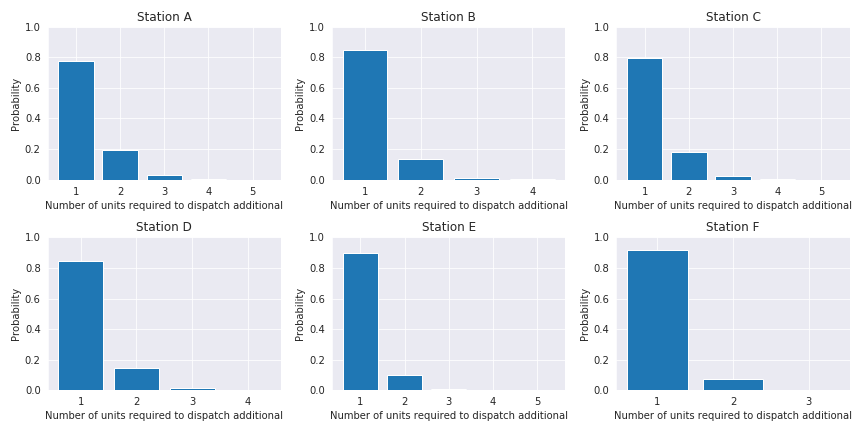
\includegraphics[width=16cm,keepaspectratio]{Figures/alsbar.png}
  \caption{Distributions of the number of ALS units required to send an additional unit at the time another ALS unit is dispatched to an incident in a station's first due area. Each of the six first due areas are shown.}
  \label{fig:alsbar}
\end{figure}

\begin{figure}[!htb]
  \centering
  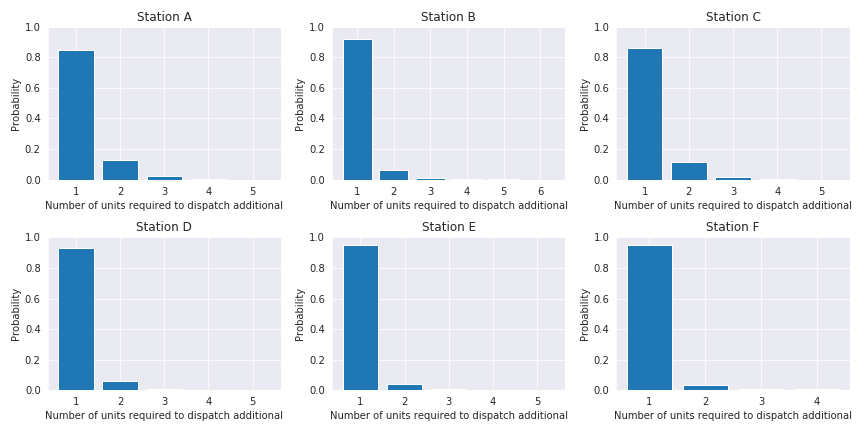
\includegraphics[width=16cm,keepaspectratio]{Figures/firebar.png}
  \caption{Distributions of the number of fire suppression units required to send an additional unit at the time another fire suppression unit is dispatched to an incident in a station's first due area. Each of the six first due areas are shown.}
  \label{fig:firebar}
\end{figure}




Using these distributions, the model can calculate the probability of a unit being sent from the first due station. This is done by Equation \ref{eq:sends_calc} for an individual station.

\begin{equation}
p_{fd} = (1-p_{down})p(N_{req} <= N_u) 
+ p_{down}p(N_{req} <= N_u-1) 
\label{eq:sends_calc}
\end{equation}


Where $p_{fd}$ is the probability that a unit is sent from the first due station, $p_{down}$ is the probability of one unit being out of service, $N_{req}$ is the number of units required to send an additional unit, and $N_u$ is the number of units belonging to a station. Note that $p(N_{req} <= N_u-1)$ and $p(N_{req} <= N_u)$ are easily computed by summing the relevant portions of the distributions shown in Figures \ref{fig:alsbar} and \ref{fig:firebar}. Note that this approach would need revision if the model were to consider cases with more than 10 units because it is not possible to have more than 10 units out of service 10\% of the time without having units out of service at the same time. The modeling approach is summarized in the influence diagram shown in Figure \ref{fig:influence}.

\begin{figure}[!htb]
  \centering
  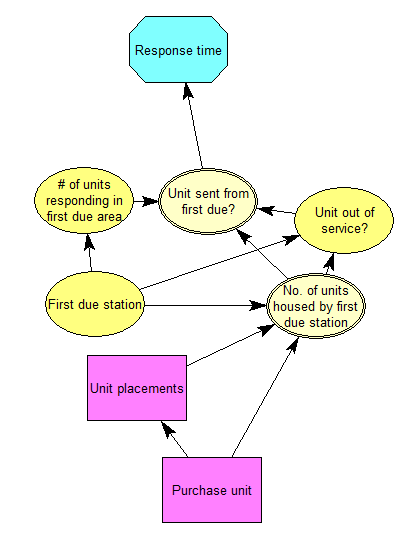
\includegraphics[width=10cm,keepaspectratio]{Figures/influence.png}
  \caption{Influence diagram summarizing the decision and modeling approach.}
  \label{fig:influence}
\end{figure}


\subsection{Distribution fitting}
For this project, several different methods of estimating hypothetical response time distributions were considered. Ideally, these methods should possess three attributes. First of all, they should be accurate, meaning that they produce estimations of the response time distributions that align with reality. Next, they should be modular, meaning that they can be easily recalculated for different modeling inputs. Finally, they should be computationally inexpensive so that an optimization routine can run many iterations in a relatively short amount of time.


The first methodology considered was a Monte-Carlo approach. This involves randomly drawing a first due station based on the observed probabilities, then randomly determining whether a unit is sent from the first due station. Note that in the Monte-Carlo simulation, this is one Bernoulli draw, rather than a set of draws corresponding to how many units are required, whether a unit is out of service, etc. Finally, a discrete uniform draw is performed over all of the response times that correspond to the drawn first due area, and whether the unit was sent from the first due station. For verification, the Monte-Carlo result is compared to the actual distribution of response times for each unit type in Figure \ref{fig:mc_comp}.

\begin{figure}[!htb]
  \centering
  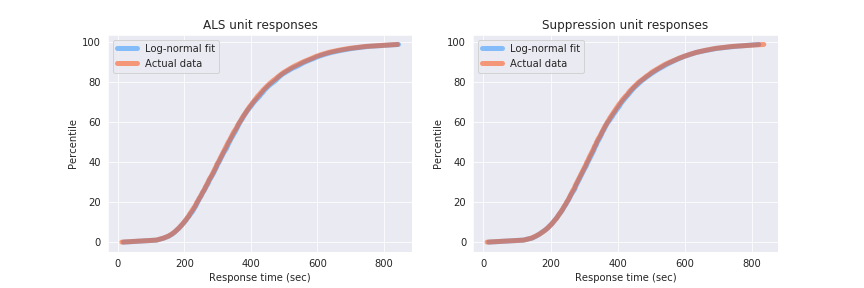
\includegraphics[width=16cm,keepaspectratio]{Figures/mccomp.png}
  \caption{A comparison of the Monte-Carlo results with 10,000 iterations to the empirical cdf for each unit type. The two curves are essentially on top of each other.}
  \label{fig:mc_comp}
\end{figure}

Although the Monte-Carlo approach is able to recreate the response time distribution nearly perfectly for both unit types, it is relatively expensive, especially considering the optimization routine must run many different cases to simulate different strategies. This motivated the exploration of other approaches to simulating the distribution. 

The next approach considered is a three-point approximation. The idea is that each of the 12 response time distributions can be approximated by three points. The well-known Swanson's mean approximation was used. This approach, first proposed by Roy Swanson in an Exxon memo in 1972, involves assigning probabilities of 0.30, 0.40, and 0.30 to the 10th, 50th, and 90th percentiles of the distribution respectively. Figure \ref{fig:swanson} shows the comparison of the Swanson's mean approximation to the empirical cdf of the full dataset. 


\begin{figure}[!htb]
  \centering
  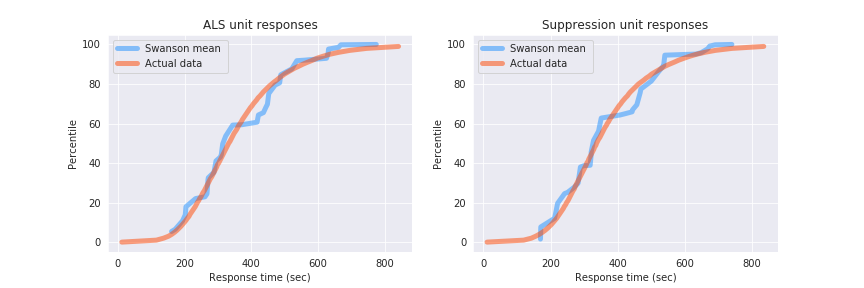
\includegraphics[width=16cm,keepaspectratio]{Figures/swanson.png}
  \caption{A comparison of the three point approximation approach (Swanson's mean) to the empirical cdf for each unit type.}
  \label{fig:swanson}
\end{figure}

Although this approach is much faster than the Monte-Carlo approach, it proved problematic when performing optimizations based on quantiles (i.e. minimizing the 90th percentile response time) because a wide interval of response times corresponded to the specified quantile. As a result, the author explored one last approach, which circumvents this issue while remaining relatively inexpensive computationally.

This approach to modeling the response time distributions is to utilize the observation reported by Buffington and Ezekoye \cite{buffington2019statistical} and Lu Lu et al. \cite{lu2014correlation} that fire department response times are well modeled by a log-normal distribution, meaning that the logarithm of response times are normally distributed. The assumption of normality is convenient because it allows for a unique characterization of the distribution by only calculating two parameters- a mean and a variance of the log-transformed response times. For a specified unit type, let $f_i$ be the probability that station $i$ is the first due station.  Then let $d_i$ be the probability that a unit came from station $i$ given that it is responding to an incident in the first due area of station $i$. From there, two vectors are constructed, $\alpha$ and $\beta$, each of containing six elements, where $\alpha_i = f_id_i$ and $\beta_i = f_i(1-d_i)$. Each entry in $\alpha$ is the joint probability of a unit responding to an incident in the first due area of station $i$ and that unit is from station $i$; conversely, each entry in $\beta$ is the joint probability of a unit responding to an incident in the first due area of station $i$ and that unit is \textit{not} from station $i$. These two vectors can be concatenated into a single vector, $w = [\alpha, \beta]^T$, of length 12, corresponding to the 12 response time distributions shown in Figure \ref{fig:alsdiff} or Figure \ref{fig:firediff}, depending on the unit type. The probability of a draw from the $j^{th}$ conditional response time distribution is therefore $w_j$. Next, the estimated mean, $\hat\mu \in R$, and the estimated variance, $\hat\sigma^2 \in R$ of the marginal log-transformed response time distribution are calculated. The calculation of the mean is relatively straightforward and is shown in Equation \ref{eq:mean_calc},


\begin{equation}
\hat\mu = w^Tm
\label{eq:mean_calc}
\end{equation}


where $m \in R^{12}$ contains the means of the log-transformed response times, which are calculated according to Equation \ref{eq:mean}:

\begin{equation}
m_j = \frac{1}{N_j}\sum_{k=1}^{N_j}log(t_{j,k})
\label{eq:mean}
\end{equation}


where $N_j$ is the number of dispatches that satisfy condition $j$, and $t_j$ is the set of reported response times corresponding to these dispatches.


In order to calculate $\hat\sigma^2$, the following variance relation is employed:


\begin{equation}
\hat\sigma^2 = \underbrace{E\big[log(t)^2\big]}_{I} - \underbrace{\bigg(E\big[log(t)\big]\bigg)^2}_{II}
\label{eq:var}
\end{equation}

Term I is then calculated according to Equation \ref{eq:mean_sq_calc}:

\begin{equation}
E\big[log(t)^2\big] = w^Tm'
\label{eq:mean_sq_calc}
\end{equation}

where 
$m'_j = \frac{1}{N_j}\sum_{k=1}^{N_j}log(t_{j,k})^2$. Term II is just the square of the mean calculated in Equation \ref{eq:mean_calc}, i.e. $\big(E\big[log(t)\big]\big)^2 = \hat\mu^2$. Once $\hat\mu$ and $\hat\sigma^2$ are calculated, they are then used to characterize a normal distribution (i.e. $ log(t) \sim N(\hat\mu, \hat\sigma^2)$), and the resulting log-normal distribution is determined by exponentiating this distribution. The cdf of the resulting log-normal distribution is shown alongside the empirical cdf for all of the reported response times in the dataset in Figure \ref{fig:lognorm}.


\begin{figure}[!htb]
  \centering
  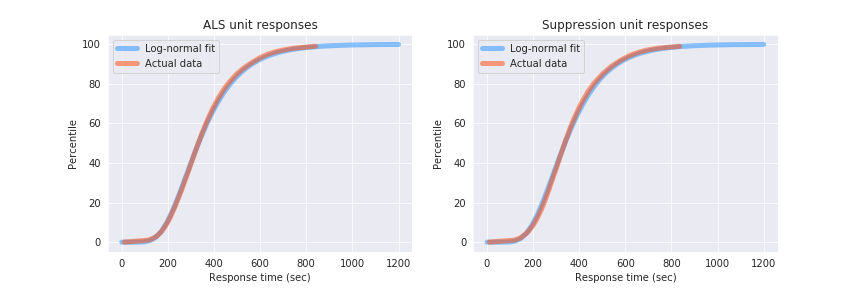
\includegraphics[width=16cm,keepaspectratio]{Figures/lognorm.png}
  \caption{A comparison of the log-normal fit to the empirical cdf for each unit type.}
  \label{fig:lognorm}
\end{figure}

This approach runs quickly and appears to reconstruct the empirical response time distribution almost perfectly, so it is the approach that is used for the optimization process described in the next section.


\section{Insights and recommendations}
The model was run to simulate every possible allocation of 2 new ALS units and 1 new fire suppression unit. It then determined the best allocation for each of these alternatives using both the mean response time and the 90th percentile response time. It found that if only one ALS unit is to be purchased, it is best to place it at station A, which would reduce the average response time for ALS units by 10 and the 90th percentile by 14 seconds. If two new ALS units are to be purchased, it is recommend that they be placed at stations A and C, which would result in an estimated reduction of 17 seconds to the mean ALS response time and a reduction of 26 seconds to the 90th percentile response time. If a fire suppression unit is purchased, placing it at station A would result in a reduction of 8 seconds to the mean fire suppression response time and a reduction of 14 seconds to the 90th percentile response time. Based on these results, and the discussions with the Business Process Analyst, it is recommended that the department purchase two new ALS units and place them at stations A and C. There appears to be little reason to purchase a new fire suppression unit for this department.


\bibliographystyle{Bibliography_Style}
\scriptsize{
\bibliography{./References}
}

\end{document}
